
\section{Usage}

From November 3, 2015 to April 11, 2016 (a period of 159 days), Skedge has seen\ldots

\begin{center}
\begin{tabular}{l}
  \hline
  4,713 users that have added or bookmarked at least one course \\ 
  5,256 schedules \\ 
  17,124 sessions\footnote{A session is defined by a period of activity expiring after 30 minutes of inactivity}, 75\% of which are from returning visitors \\ 
  107 sessions averaged per day \\ 
  5.4 pages viewed averaged per session  \\ 
  6 minutes spent averaged per session \\ 
  \hline
\end{tabular}
\end{center}

\vspace{10pt}

\noindent In this section, I will address many of the features listed in Chapter 2 (Design) and demonstrate their usability.

\subsection{Search}

\begin{figure}[H]
  \centering

  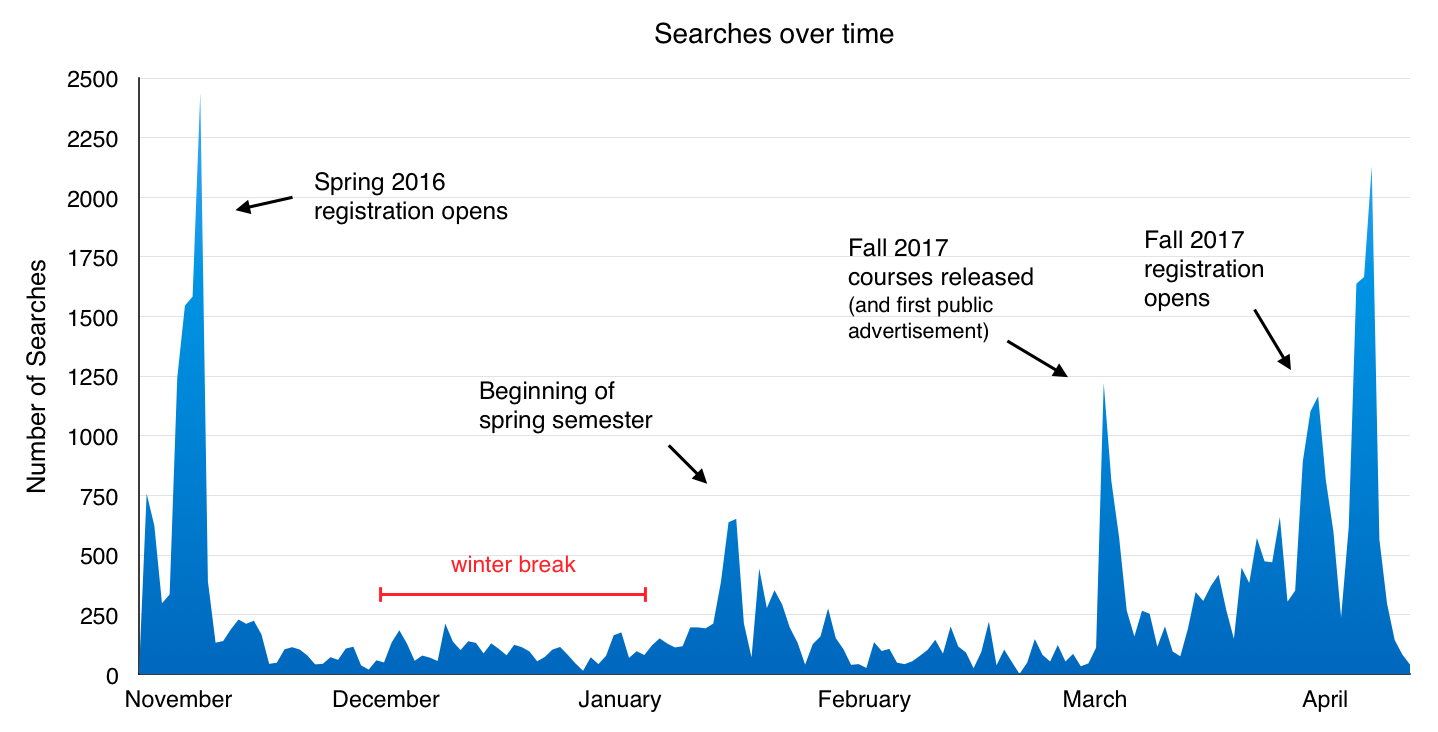
\includegraphics[width=1.0\textwidth]{images/graph/searches}

  \caption{Searches over time, with major relevant calendar events annotated}
  \label{fig:searches}

\end{figure}

Figure \ref{fig:searches} shows user search submissions over the time, and makes the periodicity of Skedge usage extremely apparent. Although it only shows a bit more than one ``phase,'' the cycle of events---\emph{semester begins} (students check course times, room locations, etc. while they get accustomed to the semester), \emph{next semester's course catalog released} (students explore the courses offered and build possible schedules), \emph{next semester registration opens} (cross-checking and officially registering each course with the Registrar)---clearly drives the majority of site traffic.

What this means is that Skedge is not seen as an experiment or a proof of concept that is not production-ready. Rather, its traffic patterns show that it is consistenly \emph{relied upon} by students and used for its intended purpose in times of biggest course scheduling need.

It should also be noted that before March, the majority of the userbase as I knew it consisted of seniors, as the majority of people that I knew personally and shared Skedge with belonged to my class. The latest two major events reported in the graph above thus very impressively consist of \emph{very few seniors}, who have no courses left to schedule. March also marked the very first time I publicly advertised Skedge, although not very strongly. It was sent out to all students in the Computer Science mailing list as well as posted to two class-wide Facebook groups.

The usability of and user satisfaction with a tool is hard to measure when it holds a monopoly. Considering that Skedge is an \emph{optional alternative} to CDCS, such consistent usage data (especially with 75\% of sessions being from returning users) undeniably prove its measures of usability and user satisfaction relative to CDCS.

  \subsubsection{Search types}

  \begin{figure}[H]
    \centering
    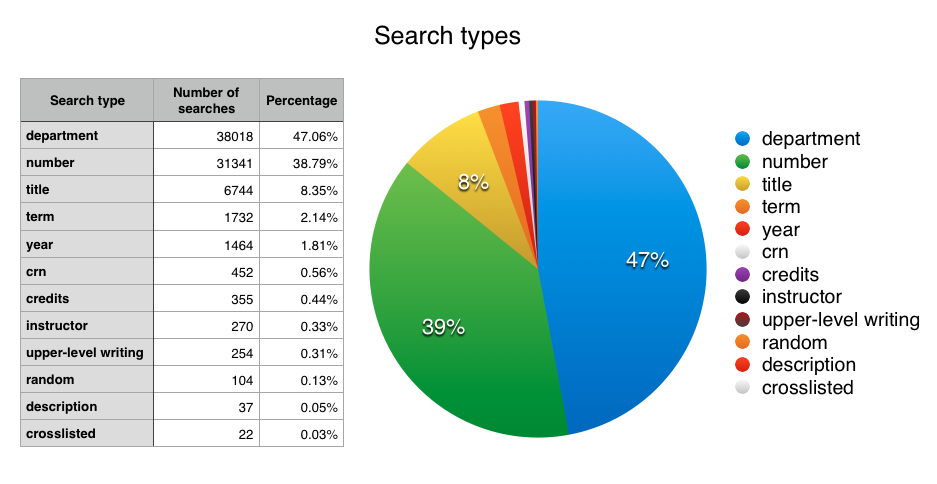
\includegraphics[width=1.0\textwidth]{images/graph/searchtypes}

    \caption{Breakdown of search queries by type of search}
    \label{fig:searchtypes}
  \end{figure}


Figure \ref{fig:searchtypes} validates the hypothesis made in Section 2.3 regarding the search interface design, demonstrating that the \emph{department code} and \emph{course number} search modes dominate user searches, accounting for over 85\% of all searches on Skedge. Bringing the nondistinct field for this in CDCS into prominence is thus a design choice that accomodates empirical usage behavior.

\subsubsection{Empty searches}

  Of the total 45,466 searches on Skedge logged since November 2nd 2015, 89.4\% (40,625) of searches produce nonempty search results, whereas 10.6\% (4,841) of searches come up empty.

  This already is evidence of an effective search mechanism, but of those empty searches, the vast majority (92\%) contain typos or are for courses that simply don't exist. The other significant portion of searches include instructor names without the requisite ``taught by'' for SkedgeQL to pick it up as an instructor search, and such a fix could easily be made.

  This type of analysis can powerfully indicate holes in the query language (i.e. searches intuitive for users) that ought to be fixed, which is the same method WolframAlpha describes its team using to improve their freeform input system \cite{wolfram2}. Table \ref{fig:empty-queries} lists a few notable examples of this nature. (Table \ref{fig:funny-queries} lists a few funny queries I came across.)

\subsection{Exports}

In Section 2.2.5 (on the design of Skedge's schedule exporting), a major usability improvement claimed was the ability to export schedules to the {\tt .ics} format, a widely used format for many calendar applications, as well as offering functional Google Calendar export. Figure \ref{fig:exports} shows usage of the export functions over time, demonstrating its consistent and healthy use (traffic surges once again in line with major scheduling events.) This data confirms that there is strong demand for exporting to {\tt .ics}---it is even more common than Google Calendar export.

\subsection{``Link-searches''}

Figure \ref{fig:linksearches} shows the amount of clicks on the Wikipedia-style embedded links throughout Skedge (instructor names link to other courses they are teaching, prerequisite and crosslist course mentions link to those courses). The number of manual instructor searches is also included for comparison, which can be seen to be vastly less usable than the analogous link-click, which doesn't exist in CDCS. Additionally, link-clicks also possibly offer a different functionality (e.g. in the course browsing paradigm).

\singlespacing
{\renewcommand{\arraystretch}{1.5}
\begin{center}
\begin{table}[H]
  \begin{tabular}{ p{6cm} p{7.5cm} }
  \hline

    ``{\tt Prereq 280}'' \newline ``{\tt has-Prereq: 280}''
    & Course dependencies \\ \hline

    ``{\tt tuesday 3:25-4:40}'' \newline ``{\tt m/w}'' \newline ``{\tt classes tuesdays and thursdays between 11:05 and 12:20}'' \newline ``{\tt weekend summer 2016}''
    & \parbox[c]{\hsize}{Better day-of-the-week handling} \\ \hline

    ``{\tt 2 credits natural science}'' 
    & Search by division (although there were very few) \\ \hline

    ``{\tt religion and classics}'' \newline ``{\tt studio art}'' 
    & Search by full department name \\ \hline

    ``{\tt new csc courses}'' 
    & The word ``{\tt courses}'' stimies the query here (somewhat common with advanced query types) \\ \hline

    ``{\tt curriculum change}'' 
    & Alternative for ``{\tt new}'' keyword \\ \hline

    ``{\tt guo}'' 
    & Instructor without ``{\tt taught by}'' (very common) \\ \hline

    ``{\tt stt212 vs mth201}'' \newline ``{\tt stt212 OR mth201}'' \newline ``{\tt csc 2\{4,8\}2}'' \newline ``{\tt csc 242|282}''
    & Searching multiple queries at the same time \\ \hline

    ``{\tt crosslisted csc lin}'' 
    & Probably a more reasonable syntax than the current SkedgeQL one (``{\tt csc x lin}'') \\ \hline

    ``{\tt place: hubbell}'' \newline ``{\tt hubbell friday}'' 
    & Search by location, although motives unclear \\ \hline

    ``{\tt MTH 2*}'' \newline ``{\tt csc 2xx}''
    & Using ``{\tt *}'' or ``{\tt x}'' instead of an omission (e.g. searching ``{\tt MTH 2}'' would work for this purpose) \\ \hline

    \hline
  \end{tabular}
  \caption{Example of search queries that produced no results but that indicate demand for added search features. The corresponding features that currently lack in SkedgeQL are described on the right.}
  \label{fig:empty-queries}
\end{table}

\vspace{30pt}

\begin{table}[H]
  \begin{tabular}{ | p{4cm} | p{4cm} | p{4cm} | }
  \hline

    ``{\tt Larry david}''
    & ``{\tt taught by seligman}''
    & ``{\tt cool stuff}''
    \\ \hline

    ``{\tt game of thrones}''
    & ``{\tt interesting courses}''
    & ``{\tt fun classes in csc}''
    \\ \hline
    

    ``{\tt easy A}''
    & ``{\tt flute birdman}''
    & ``{\tt how do i make a new schedule}''
    \\ \hline

    \hline
  \end{tabular}
  \caption{Humorous search submissions}
  \label{fig:funny-queries}
\end{table}
\end{center}

\doublespacing

\begin{figure}[H]
  \centering
  \vspace{20pt}
    \begin{subfigure}[w]{14cm}
      \centering
      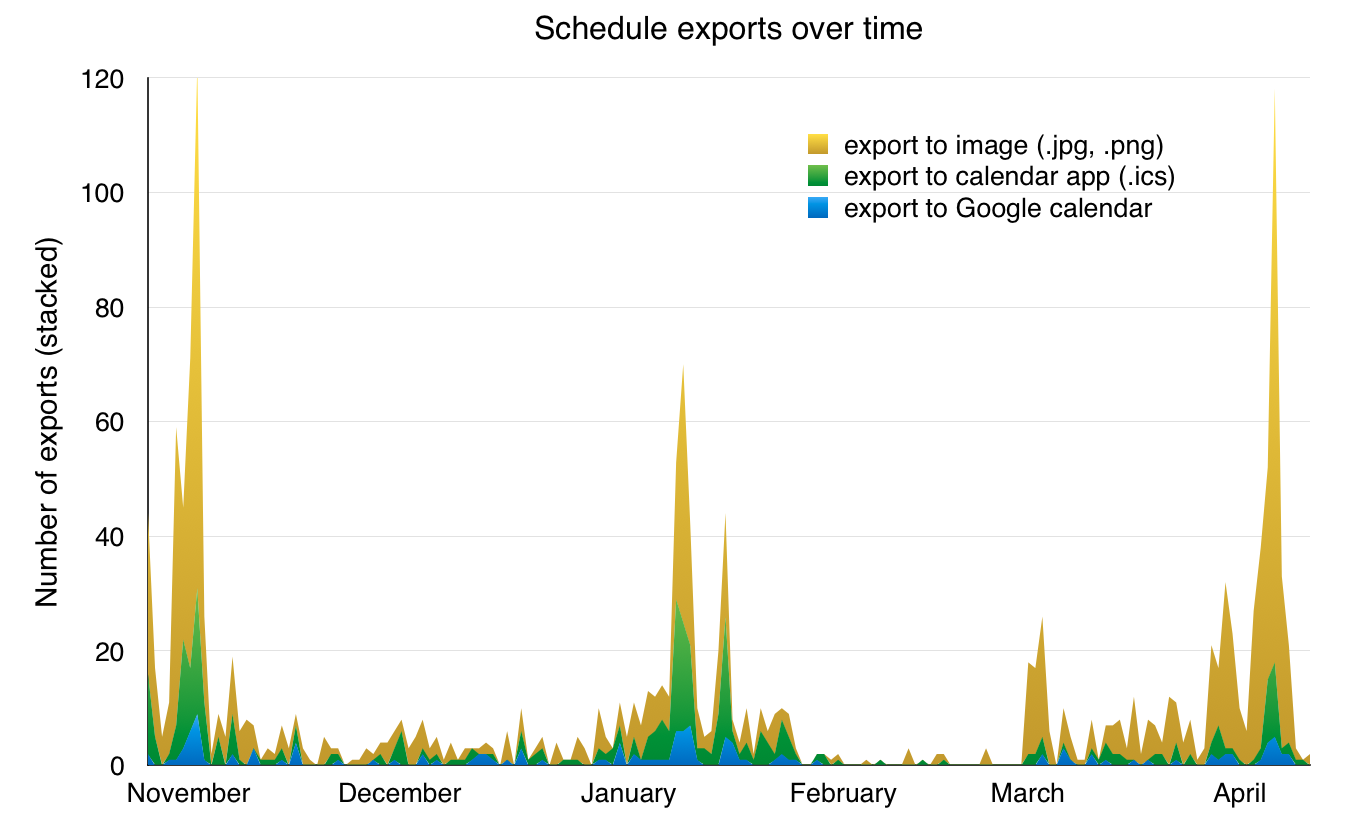
\includegraphics[width=1.00\textwidth]{images/graph/exports}
      \caption{Different types of schedule exporting over time} \label{fig:exports}
    \end{subfigure} \\
    \vspace{30pt}
    \begin{subfigure}[w]{14cm}
      \centering
      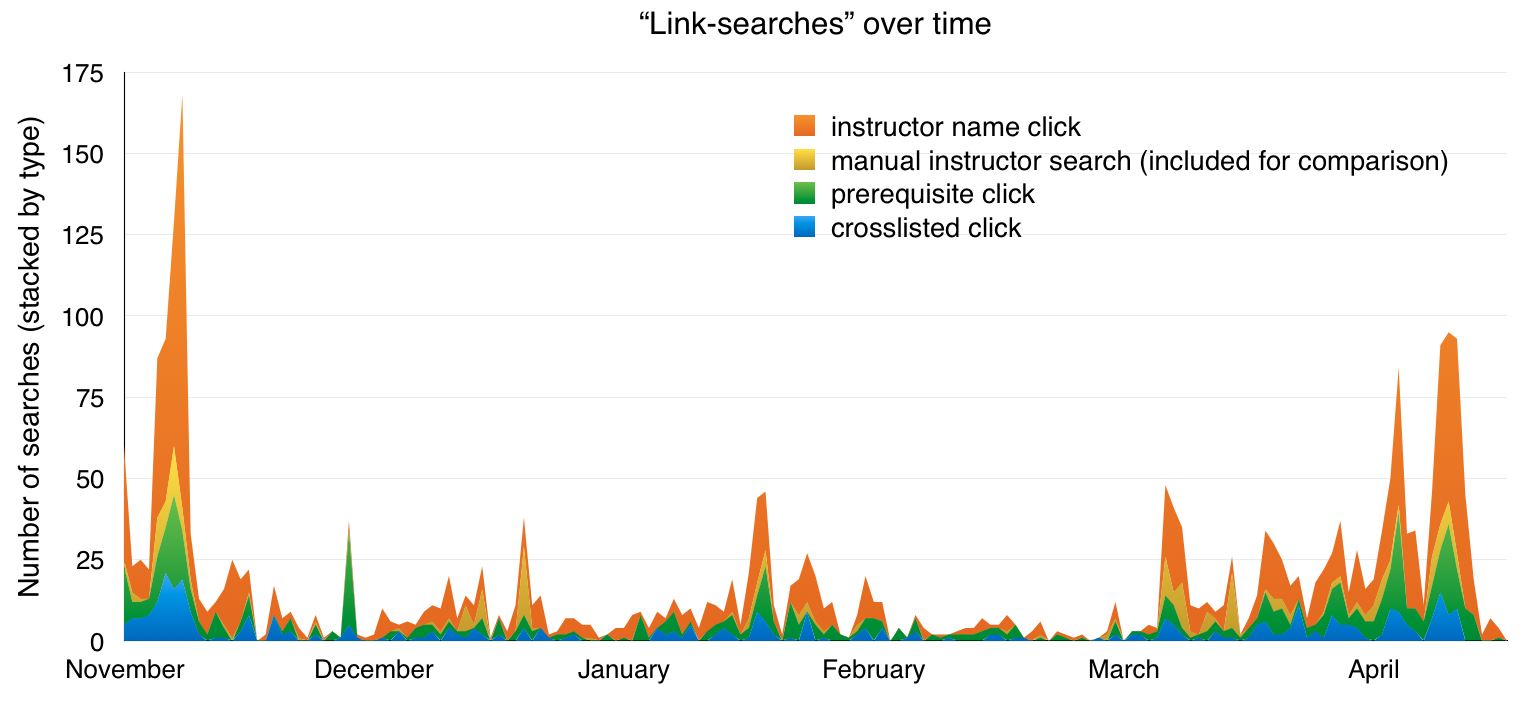
\includegraphics[width=1.00\textwidth]{images/graph/linksearches}
      \caption{Different types of ``link-search'' clicks over time, with manual instructor search included for comparison with clicking on an instructor's name} \label{fig:linksearches}
    \end{subfigure}

  \caption{Other metrics of Skedge usage over time}
\end{figure}

\clearpage

\subsection{Mobile}

Making the case for usability superior to CDCS's in the space of mobile support is easy, given that CDCS does not have a mobile-responsive website. But to illustrate the importance of ensuring good user experience on mobile devices, consder that 11.54\% of all Skedge sessions are from mobile devices, which is very substantial. On average, 2.74 pages viewed are viewed and 2 minutes are spent per session on mobile devices.

The nature of the content also makes Skedge commonly accessed on the go---quickly looking up room numbers while heading to class, for instance, or checking a friend's schedule on Skedge Social to meet them after a class, etc. There is still work to be done to determine the usability of Skedge's mobile site in particular. Surveys could be a good indicator, but I didn't have the chance to administer any.


\subsection{Course blocks}

\begin{figure}[H]
  \centering

  \fbox {
    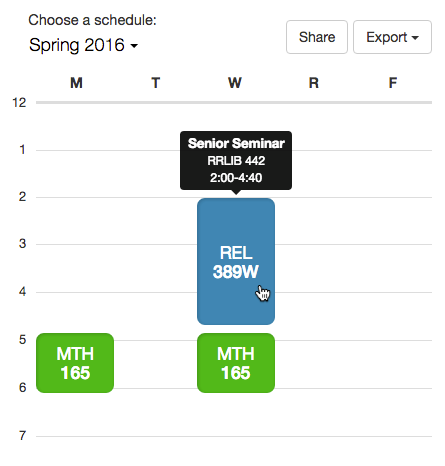
\includegraphics[width=8cm]{images/skedge/blocks}
  }

  \caption{Etc}
  \label{fig:searchtypes}

\end{figure}

40\% of sessions have at least one block-click
Average of 5.12 block-clicks per session

success because you can't click schedule blocks in better cdcs!!